\documentclass[a4paper,14pt]{extreport}
	\usepackage[left=1.5cm,right=1.5cm,
	    top=1.5cm,bottom=2cm,bindingoffset=0cm]{geometry}
	\usepackage{scrextend}
	\usepackage[T1,T2A]{fontenc}
	\usepackage[utf8]{inputenc}
	\usepackage[english,russian,ukrainian]{babel}
	\usepackage{tabularx}
	\linespread{1.5}
	\usepackage{amssymb}
	\usepackage{color}
	\usepackage{amsmath}
	\usepackage{mathrsfs}
	\usepackage{listings}
	\usepackage{graphicx}
	\graphicspath{ {./images/} }
	\usepackage{lipsum}
	\usepackage{xcolor}
	\usepackage{hyperref}
	\usepackage{tcolorbox}
	\usepackage{tikz}
	\usepackage[framemethod=TikZ]{mdframed}
	\usepackage{wrapfig,boxedminipage,lipsum}
	\mdfdefinestyle{MyFrame}{%
	linecolor=blue,outerlinewidth=2pt,roundcorner=20pt,innertopmargin=\baselineskip,innerbottommargin=\baselineskip,innerrightmargin=20pt,innerleftmargin=20pt,backgroundcolor=gray!50!white}
	 \usepackage{csvsimple}
	 \usepackage{supertabular}
	\usepackage{pdflscape}
	\usepackage{fancyvrb}
	%\usepackage{comment}
	\usepackage{array,tabularx}
	\usepackage{colortbl}

	\usepackage{varwidth}
	\tcbuselibrary{skins}
	\usepackage{fancybox}
	\usepackage{multicol}
	\usepackage{multirow}
	\usepackage{pgfplots}
	\pgfplotsset{compat=1.9}


	\usepackage{tikz}
	\usepackage[framemethod=TikZ]{mdframed}
	\usepackage{xcolor}
	\usetikzlibrary{calc}
	\makeatletter
	\newlength{\mylength}
	\xdef\CircleFactor{1.1}
	\setlength\mylength{\dimexpr\f@size pt}
	\newsavebox{\mybox}
	\newcommand*\circled[2][draw=blue]{\savebox\mybox{\vbox{\vphantom{WL1/}#1}}\setlength\mylength{\dimexpr\CircleFactor\dimexpr\ht\mybox+\dp\mybox\relax\relax}\tikzset{mystyle/.style={circle,#1,minimum height={\mylength}}}
	\tikz[baseline=(char.base)]
	\node[mystyle] (char) {#2};}
	\makeatother

	\definecolor{ggreen}{rgb}{0.4,1,0}
	\definecolor{rred}{rgb}{1,0.1,0.1}
	\definecolor{amber}{rgb}{1.0, 0.75, 0.0}
	\definecolor{babyblue}{rgb}{0.54, 0.81, 0.94}
	\definecolor{amethyst}{rgb}{0.6, 0.4, 0.8}

	\usepackage{float}
	\usepackage{wrapfig}
	\usepackage{framed}
	%for nice Code{
	\lstdefinestyle{customc}{
	  belowcaptionskip=1\baselineskip,
	  breaklines=true,
	  frame=L,
	  xleftmargin=\parindent,
	  language=C,
	  showstringspaces=false,
	  basicstyle=\small\ttfamily,
	  keywordstyle=\bfseries\color{green!40!black},
	  commentstyle=\itshape\color{purple!40!black},
	  identifierstyle=\color{blue},
	  stringstyle=\color{orange},
	}
\lstset{escapechar=@,style=customc}
%}
%----------------------------------------%----------------------------------------%----------------------------------------%----------------------------------

\begin{document}
\pagecolor{white}

%----------------------------------------1
\newtcbox{\xmybox}[1][red]{on line, arc=7pt,colback=#1!10!white,colframe=#1!50!black, before upper={\rule[-3pt]{0pt}{10pt}},boxrule=1pt, boxsep=0pt,left=6pt,right=6pt,top=2pt,bottom=2pt}

\begin{titlepage}
  \begin{center}
    \large
    Національний технічний університет України \\ "Київський політехнічний інститут імені Ігоря Сікорського"


    Факультет Електроніки

    Кафедра мікроелектроніки
    \vfill

    \textsc{ЗВІТ}\\

    {\Large Про виконання лабораторної роботи №4\\
      з дисципліни: «Схемотехніка-1»\\[1cm]

        Активнi RC-фiльтри


	    }
	  \bigskip
	\end{center}
	\vfill

	\newlength{\ML}
	\settowidth{\ML}{«\underline{\hspace{0.4cm}}» \underline{\hspace{2cm}}}
	\hfill
	\begin{minipage}{1\textwidth}
	Виконавець:\\
	Студент 3-го курсу \hspace{4cm} $\underset{\text{(підпис)}}{\underline{\hspace{0.2\textwidth}}}$  \hspace{1cm}А.\,С.~Мнацаканов\\
	\vspace{1cm}

	Перевірила: \hspace{6.1cm} $\underset{\text{(підпис)}}{\underline{\hspace{0.2\textwidth}}}$  \hspace{1cm}Г.\,С.~Порева\\

	\end{minipage}

	\vfill

	\begin{center}
	2021
	\end{center}
\end{titlepage}


\begin{center}Мета роботи\end{center}\par
Вивчення принципiв роботи, дослiдження амплiтудних та частотних характеристик i параметрiв активних RC-фiльтрiв нижнiх та верхнiх частот, полоснопропускаючого та полосно-затримуючого фiльтрiв на iнтегральному операцiйному пiдсилювачi.

\begin{figure}[h]
	\center{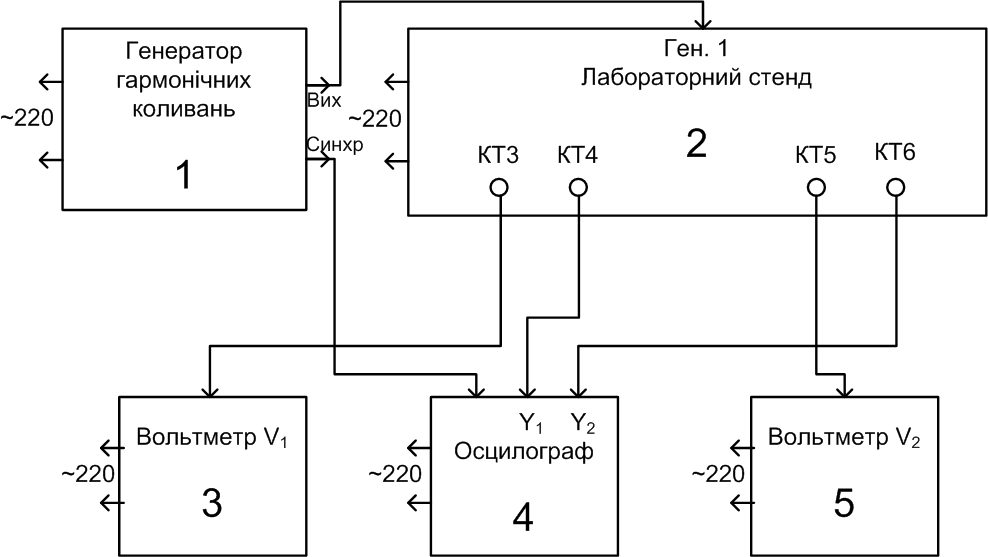
\includegraphics[width=0.8\linewidth]{sxema.png}}
	\caption{ Блок-схема установки для дослідження лабораторного модуля «АRC-фільтр».}
\end{figure}\par

\begin{landscape}
	\begin{figure}[h]
		\center{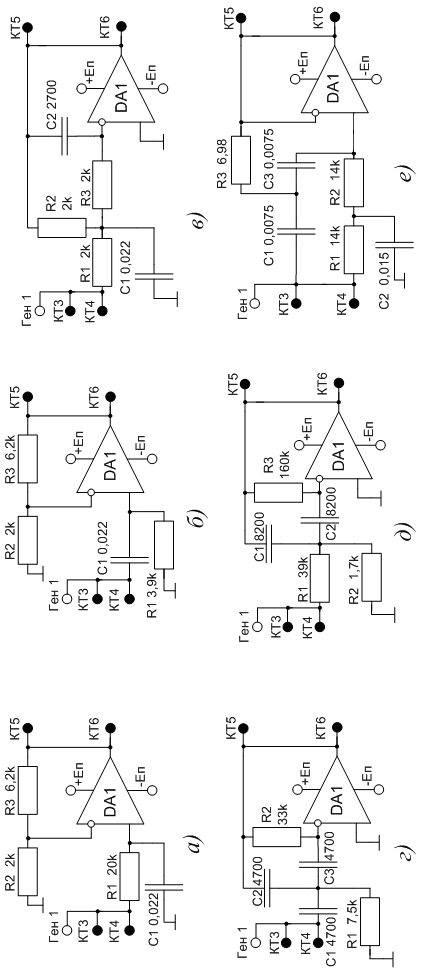
\includegraphics[angle = -90, width=0.8\linewidth]{s1.png}}
		\caption{Схема електрична принципова лабораторного модуля «АRC фільтри»: а) схема ФНЧ-1 (П1-вкл), б) схема ФВЧ-1 (П2-вкл), в) схема ФНЧ-2 (П3-вкл), г) схема ФВЧ-2 (П4-вкл), д) схема ПФ-2 (П5-вкл), е) схема ЗФ-2 (П6-вкл).}
	\end{figure}
\end{landscape}




\begin{table}[h!]%        ФНЧ
	\begin{center}
		\begin{small}
			\begin{tabular}{|c|c|c|c|c|c|c|c|c|c|}
			\hline
			\multicolumn{10}{|c|}{ФНЧ}             \\ \hline
			\multicolumn{5}{|c|}{ФНЧ-1} & \multicolumn{5}{c|}{ФНЧ-2}       \\ \hline
			$f$, Гц  & U2, мB & lg $f$ & Ku           & $\varphi$           & $f$, Гц & U2, мB & lg$ f$ & Ku   & $\varphi$     \\ \hline
			20     & 2000   & 1.30 & 4.00         & 0           & 20    & 500    & 1.30 & 1    & 180   \\ \hline
			100    & 1950   & 2.00 & 3.90         & 14.2        & 500   & 500    & 2.70 & 1    &       \\ \hline
			150    & 1860   & 2.18 & 3.72         &             & 1000  & 500    & 3.00 & 1    & 180   \\ \hline
			200    & 1760   & 2.30 & 3.52         & 36          & 5000  & 533    & 3.70 & 1.06 & 158   \\ \hline
			300    & 1540   & 2.48 & 3.08         &             & 10000 & 480    & 4.00 & 0.96 & 90    \\ \hline
			500    & 1160   & 2.70 & 2.32         &             & 13000 & 345    & 4.11 & 0.69 &       \\ \hline
			1000   & 675    & 3.00 & 1.35         & 72          & 15000 & 270    & 4.18 & 0.54 &       \\ \hline
			2000   & 357    & 3.30 & 0.71         & 86.4        & 20000 & 150    & 4.30 & 0.3  & 36    \\ \hline
			5000   & 145    & 3.70 & 0.29         &             & 30000 & 65     & 4.48 & 0.13 & 14.4  \\ \hline
			10000  & 76     & 4.00 & 0.15         & 86.4        & 50000 & 20     & 4.70 & 0.04 &       \\ \hline
			$fc$  & \multicolumn{4}{c|}{360 Гц}     & $fc $			& \multicolumn{4}{c|}{13 кГц}          \\ \hline
			$\triangle f$ & \multicolumn{4}{c|}{360 Гц} & $\triangle f$ & \multicolumn{4}{c|}{13 кГц}		   \\ \hline
			Д & \multicolumn{4}{c|}{1440}& Д & \multicolumn{4}{c|}{13.75 $\cdot 10^3$} \\ \hline
			\end{tabular}
		\end{small}
	\end{center}
\end{table}

\begin{table}[h!]%        ФBЧ
	\begin{center}
		\begin{small}
			\begin{tabular}{|c|c|c|c|c|c|c|c|c|c|}
			\hline
			\multicolumn{10}{|c|}{ФВЧ}                                                      \\ \hline
			\multicolumn{5}{|c|}{ФВЧ}              & \multicolumn{5}{c|}{ФВЧ}               \\ \hline
			$f$, Гц & $lg f$ & U2, мВ & $K_u$ & $\varphi$    & $f$, Гц & $lg f$ & $U_2$, мВ & $K_u $  & $\varphi$     \\ \hline
			20      & 1.30 & 10     & 0.02  & 81   & 20      & 1.30 & 8      & 1.30 &       \\ \hline
			100     & 2.00 & 115    & 0.23  & 82.8 & 200     & 2.30 & 3.5    & 2.30 & 7.2   \\ \hline
			500     & 2.70 & 545    & 1.09  & 72   & 500     & 2.70 & 22.4   & 2.70 & 14.4  \\ \hline
			1000    & 3.00 & 980    & 1.96  & 57.6 & 1000    & 3.00 & 88     & 3.00 & 36    \\ \hline
			2000    & 3.30 & 1500   & 3     & 43.2 & 1500    & 3.18 & 184    & 3.18 &       \\ \hline
			3000    & 3.48 & 1720   & 3.44  & 21.6 & 2000    & 3.30 & 286    & 3.30 & 79.2  \\ \hline
			5000    & 3.70 & 1890   & 3.78  &      & 3000    & 3.48 & 408    & 3.48 &       \\ \hline
			8000    & 3.9  & 1960   & 3.92  & 7.2  & 4000    & 3.60 & 452    & 3.60 & 129.6 \\ \hline
			15000   & 4.18 & 2000   & 4     &      & 5000    & 3.7  & 471    & 3.70 & 162   \\ \hline
			20000   & 4.30 & 2000   & 4     & 0    & 20000   & 4.30 & 485    & 4.30 & 172.8 \\ \hline
			$f_c $     & \multicolumn{4}{c|}{1800 Гц} & $f_c$      & \multicolumn{4}{c|}{2350 Гц} \\ \hline
			\end{tabular}
		\end{small}
	\end{center}
\end{table}

\begin{table}[]% 		 ПФ ЗФ
	\begin{center}
		
			\begin{tabular}{|c|c|c|c|c|c|c|c|c|c|}
			\hline
			\multicolumn{5}{|c|}{ПФ-2}               & \multicolumn{5}{c|}{ЗФ-2}                  \\ \hline
			f, Tu      & U2, mB & lg f & Ku   & $\varphi$    & f, Til     & U2, mB  & lg f & Ku   & $\varphi$     \\ \hline
			20         & 5.13   & 1.30 & 0.01 & 86.4 & 100        & 496     & 2.00 & 0.99 & 0     \\ \hline
			500        & 90     & 2.70 & 0.18 & 93.6 & 200        & 485     & 2.30 & 0.97 & 14.4  \\ \hline
			600        & 116    & 2.78 & 0.23 &      & 500 (400)  & 413     & 2.70 & 0.83 & 28.8  \\ \hline
			800        & 192    & 2.90 & 0.38 &      & 800        & 303     & 2.90 & 0.61 &       \\ \hline
			900        & 253    & 2.95 & 0.51 &      & 1000       & 225     & 3.00 & 0.45 & 61.2  \\ \hline
			1000       & 345    & 3.00 & 0.69 & 108  & 1200       & 145     & 3.08 & 0.29 &       \\ \hline
			1200       & 748    & 3.08 & 1.50 &      & 1500       & 39.2    & 3.18 & 0.08 &       \\ \hline
			1500       & 580    & 3.18 & 1.16 &      & 2000       & 103     & 3.30 & 0.21 & 288   \\ \hline
			2000       & 228    & 3.30 & 0.46 & 252  & 5000       & 401     & 3.70 & 0.80 & 316.8 \\ \hline
			3000       & 110    & 3.48 & 0.22 & 252  & 10000      & 472     & 4.00 & 0.94 & 345.6 \\ \hline
			$f_0$      & \multicolumn{4}{c|}{1.3 кГц}    & $f_0$      & \multicolumn{4}{c|}{1.6 кГц}     \\ \hline
			$f_n$      & \multicolumn{4}{c|}{1.17 Гц}   & $f_n$      & \multicolumn{4}{c|}{6741 Гц}    \\ \hline
			$f_B$      & \multicolumn{4}{c|}{1.45 кГц}   & $f_B$      & \multicolumn{4}{c|}{3.980 кГц}    \\ \hline
			$\triangle f$ & \multicolumn{4}{c|}{150 кГц}    & $\triangle f$ & \multicolumn{4}{c|}{3.306 кГц}   \\ \hline
			Д          & \multicolumn{4}{c|}{283.5}  & Д          & \multicolumn{4}{c|}{3273} \\ \hline
			\end{tabular}
		
	\end{center}
\end{table}

\clearpage
\newpage
\begin{center}
	Графіки
\end{center}


\begin{figure}[h!]
	\centering
	\begin{tikzpicture}
		\begin{axis}[table/col sep = semicolon,
			title=ФНЧ-1,
			xlabel = $lg f$,
    		ylabel = {$K_u$},
			height = 0.3\paperheight, 
			width = 0.3\paperwidth,
			/pgf/number format/1000 sep={}]
		\addplot table [grid style = both, x={c}, y={d}] {tt1.csv};
		\end{axis}		
	\end{tikzpicture}
	\hspace{2cm}
	\begin{tikzpicture}
		\begin{axis}[table/col sep = semicolon,
		title=ФНЧ-2,
		xlabel = $lg f$,
		ylabel = {$K_u$},
		height = 0.3\paperheight, 
		width = 0.3\paperwidth,
		/pgf/number format/1000 sep={}]
		\addplot table [grid style = both, x={h}, y={i}] {tt1.csv};
		\end{axis}		
	\end{tikzpicture}
%\caption{ФНЧ}
\end{figure}

\begin{figure}[h!]
	\centering
	\begin{tikzpicture}
		\begin{axis}[table/col sep = semicolon,
			title=ФВЧ-1,
			xlabel = $lg f$,
    		ylabel = {$K_u$},
			height = 0.3\paperheight, 
			width = 0.3\paperwidth,
			/pgf/number format/1000 sep={}]
		\addplot table [grid style = both, x={a}, y={b}] {tab2n.csv};
		\end{axis}		
	\end{tikzpicture}
	\hspace{2cm}
	\begin{tikzpicture}
		\begin{axis}[table/col sep = semicolon,
		title=ФВЧ-2,
		xlabel = $lg f$,
		ylabel = {$K_u$},
		height = 0.3\paperheight, 
		width = 0.3\paperwidth,
		/pgf/number format/1000 sep={}]
		\addplot table [grid style = both, x={d}, y={e}] {tab2n.csv};
		\end{axis}		
	\end{tikzpicture}
%\caption{ФВЧ}
\end{figure}

\begin{figure}[h!]
	\centering
	\begin{tikzpicture}
		\begin{axis}[table/col sep = semicolon,
			title=ПФ-2,
			xlabel = $lg f$,
    		ylabel = {$K_u$},
			height = 0.3\paperheight, 
			width = 0.3\paperwidth,
			/pgf/number format/1000 sep={}]
		\addplot table [grid style = both, x={a}, y={b}] {tab3n.csv};
		\end{axis}		
	\end{tikzpicture}
	\hspace{2cm}
	\begin{tikzpicture}
		\begin{axis}[table/col sep = semicolon,
		title=ЗВ-2,
		xlabel = $lg f$,
		ylabel = {$K_u$},
		height = 0.3\paperheight, 
		width = 0.3\paperwidth,
		/pgf/number format/1000 sep={}]
		\addplot table [grid style = both, x={d}, y={e}] {tab3n.csv};
		\end{axis}		
	\end{tikzpicture}
%\caption{ПФ ЗВ}
\end{figure}


%///////////////////
%///////////////////
\clearpage
\newpage
\noindent{\color{red} \rule{\linewidth}{1mm} }
\begin{figure}[h!]
	\centering
	\begin{tikzpicture}
		\begin{axis}[table/col sep = semicolon,
			title=ФНЧ-1,
			xlabel = $lg f$,
    		ylabel = {$\varphi$},
			height = 0.3\paperheight, 
			width = 0.3\paperwidth,
			/pgf/number format/1000 sep={}]
		\addplot table [grid style = both, x={c}, y={e}] {tt1.csv};
		\end{axis}		
	\end{tikzpicture}
	\hspace{2cm}
	\begin{tikzpicture}
		\begin{axis}[table/col sep = semicolon,
		title=ФНЧ-2,
		xlabel = $lg f$,
		ylabel = {$\varphi$},
		height = 0.3\paperheight, 
		width = 0.3\paperwidth,
		/pgf/number format/1000 sep={}]
		\addplot table [grid style = both, x={h}, y={j}] {tt1.csv};
		\end{axis}		
	\end{tikzpicture}
\end{figure}

\begin{figure}[h!]
	\centering
	\begin{tikzpicture}
		\begin{axis}[table/col sep = semicolon,
			title=ФВЧ-1,
			xlabel = $lg f$,
    		ylabel = {$\varphi$},
			height = 0.3\paperheight, 
			width = 0.3\paperwidth,
			/pgf/number format/1000 sep={}]
		\addplot table [grid style = both, x={a}, y={c}] {tab2n.csv};
		\end{axis}		
	\end{tikzpicture}
	\hspace{2cm}
	\begin{tikzpicture}
		\begin{axis}[table/col sep = semicolon,
		title=ФВЧ-2,
		xlabel = $lg f$,
		ylabel = {$\varphi$},
		height = 0.3\paperheight, 
		width = 0.3\paperwidth,
		/pgf/number format/1000 sep={}]
		\addplot table [grid style = both, x={d}, y={f}] {tab2n.csv};
		\end{axis}		
	\end{tikzpicture}
\end{figure}

\begin{figure}[h!]
	\centering
	\begin{tikzpicture}
		\begin{axis}[table/col sep = semicolon,
			title=ПФ-1,
			xlabel = $lg f$,
    		ylabel = {$\varphi$},
			height = 0.3\paperheight, 
			width = 0.3\paperwidth,
			/pgf/number format/1000 sep={}]
		\addplot table [grid style = both, x={a}, y={c}] {tab3n.csv};
		\end{axis}		
	\end{tikzpicture}
	\hspace{2cm}
	\begin{tikzpicture}
		\begin{axis}[table/col sep = semicolon,
		title=ЗВ-2,
		xlabel = $lg f$,
		ylabel = {$\varphi$},
		height = 0.3\paperheight, 
		width = 0.3\paperwidth,
		/pgf/number format/1000 sep={}]
		\addplot table [grid style = both, x={d}, y={f}] {tab3n.csv};
		\end{axis}		
	\end{tikzpicture}
\end{figure}


\clearpage
\newpage


\begin{figure}[h]
	\center{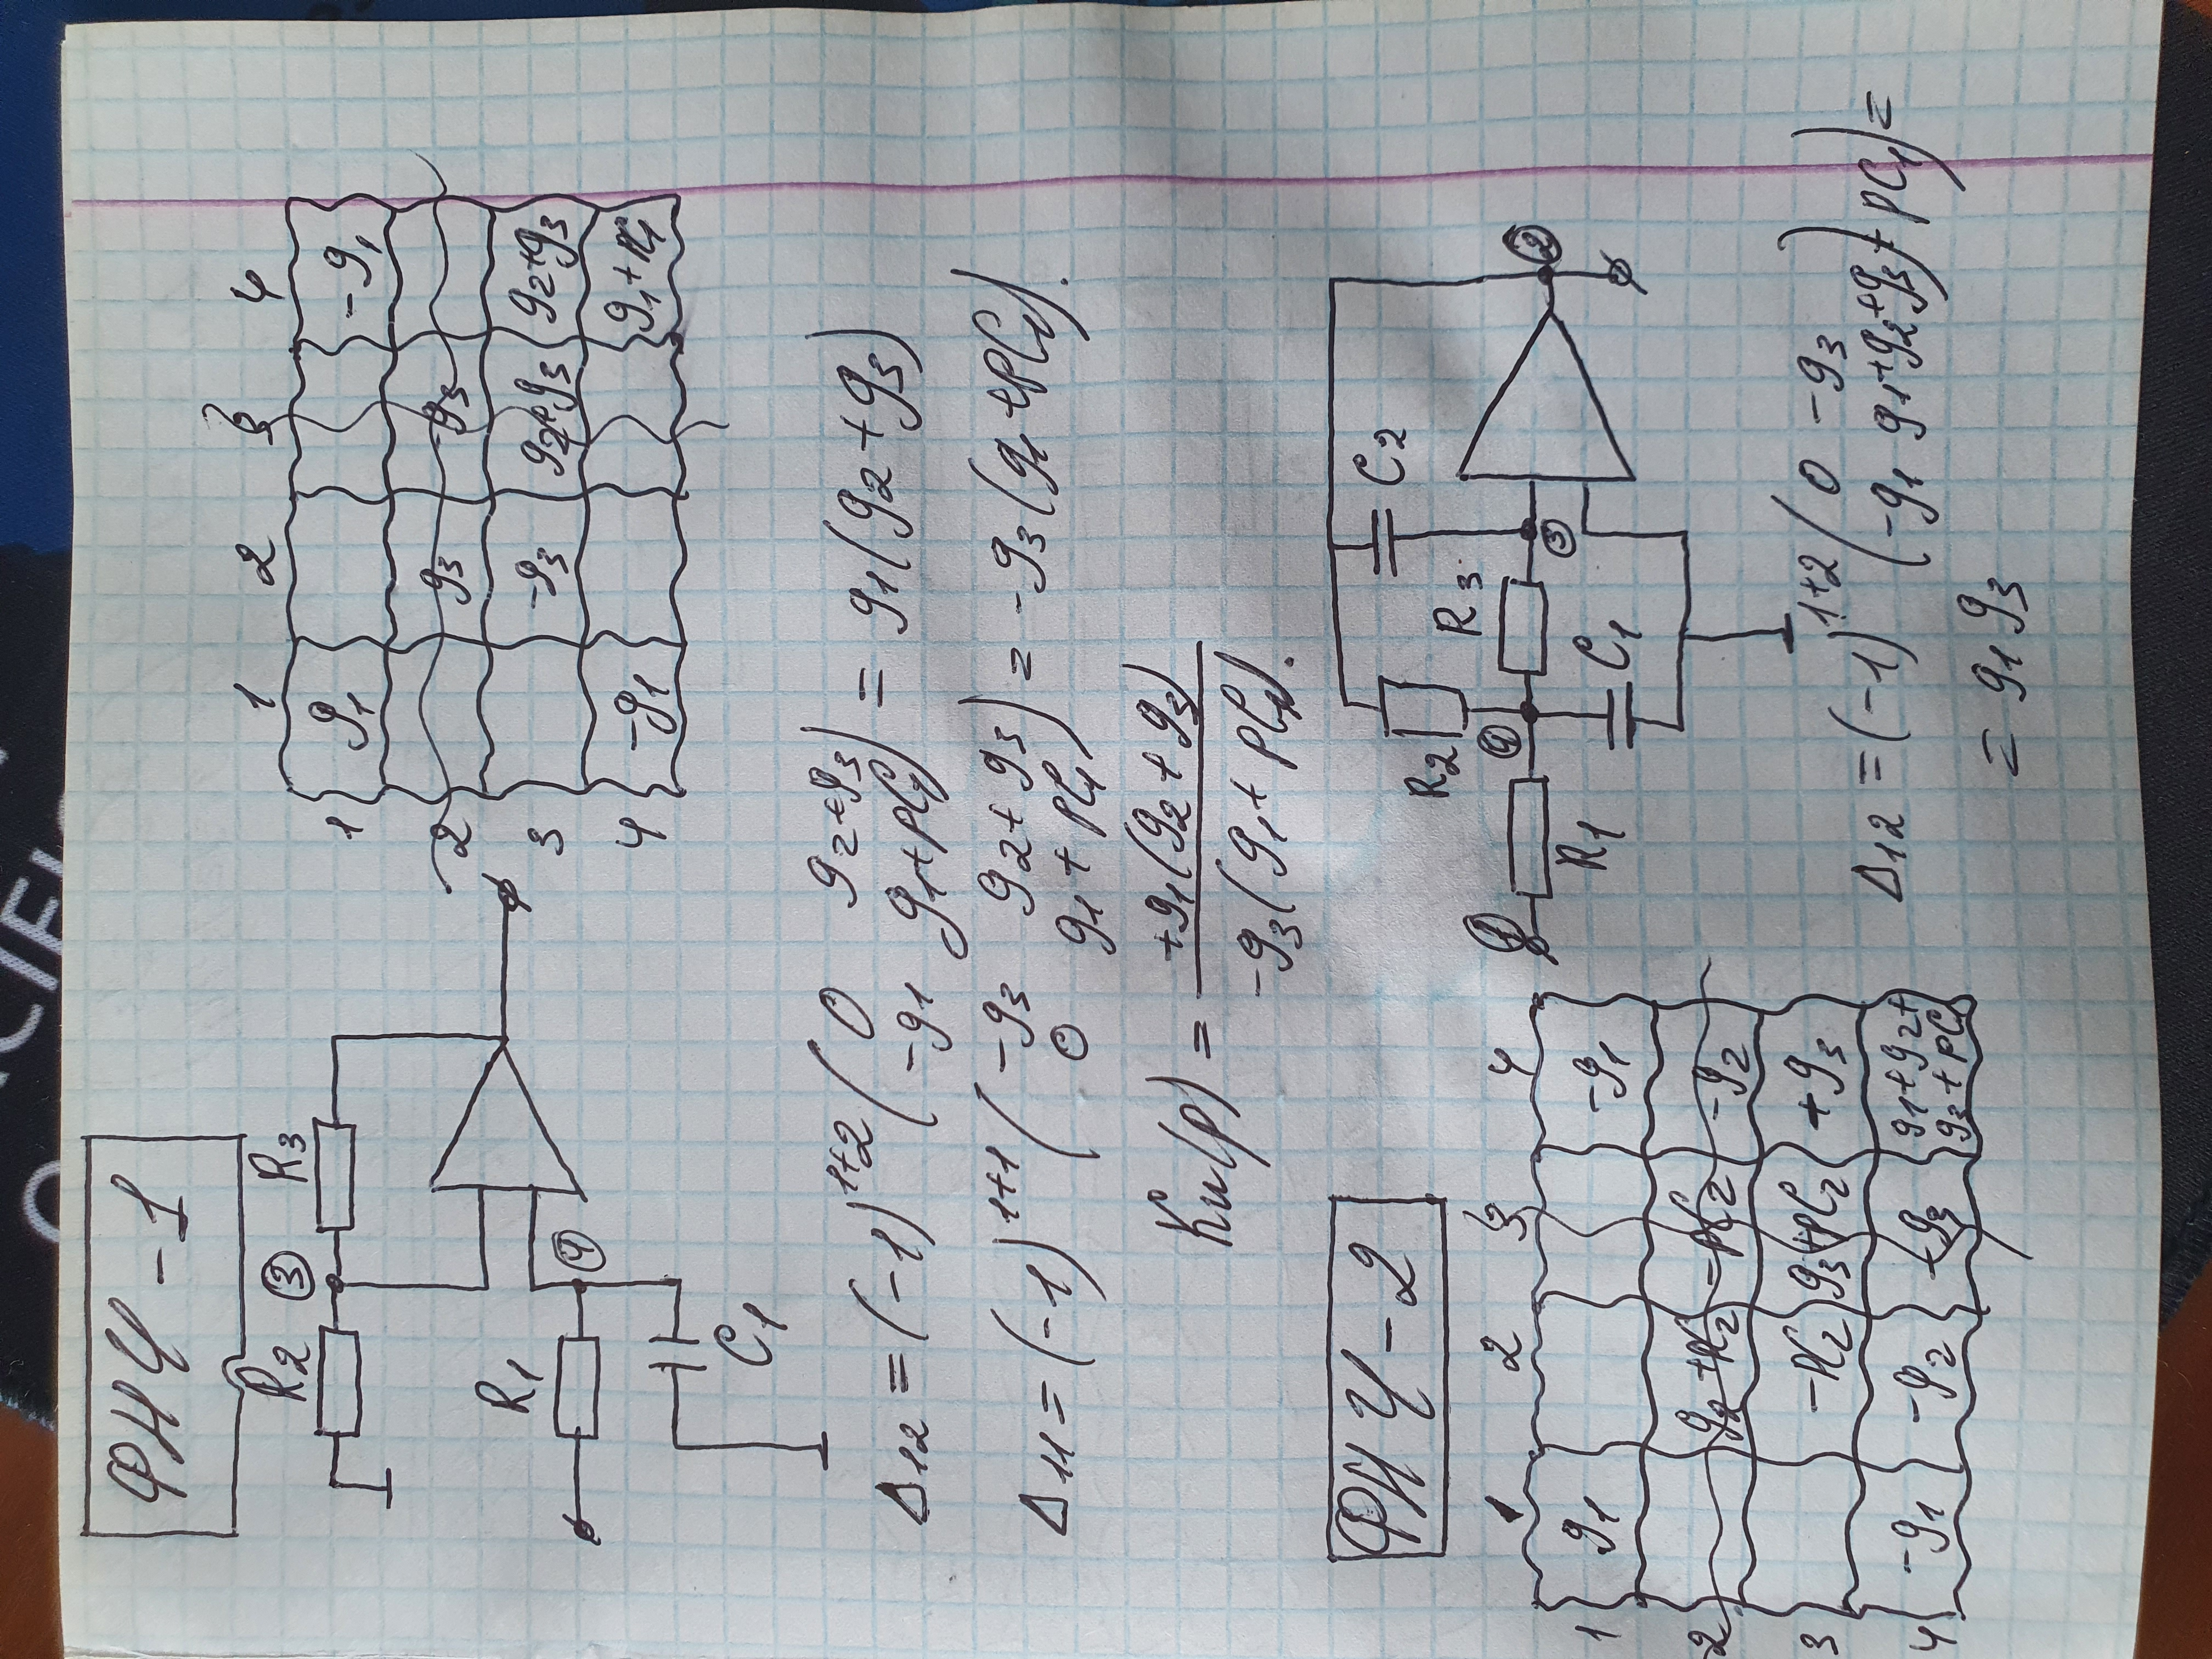
\includegraphics[angle = -90, width=0.8\linewidth]{1.jpg}}
\end{figure}

\begin{figure}[h]
	\center{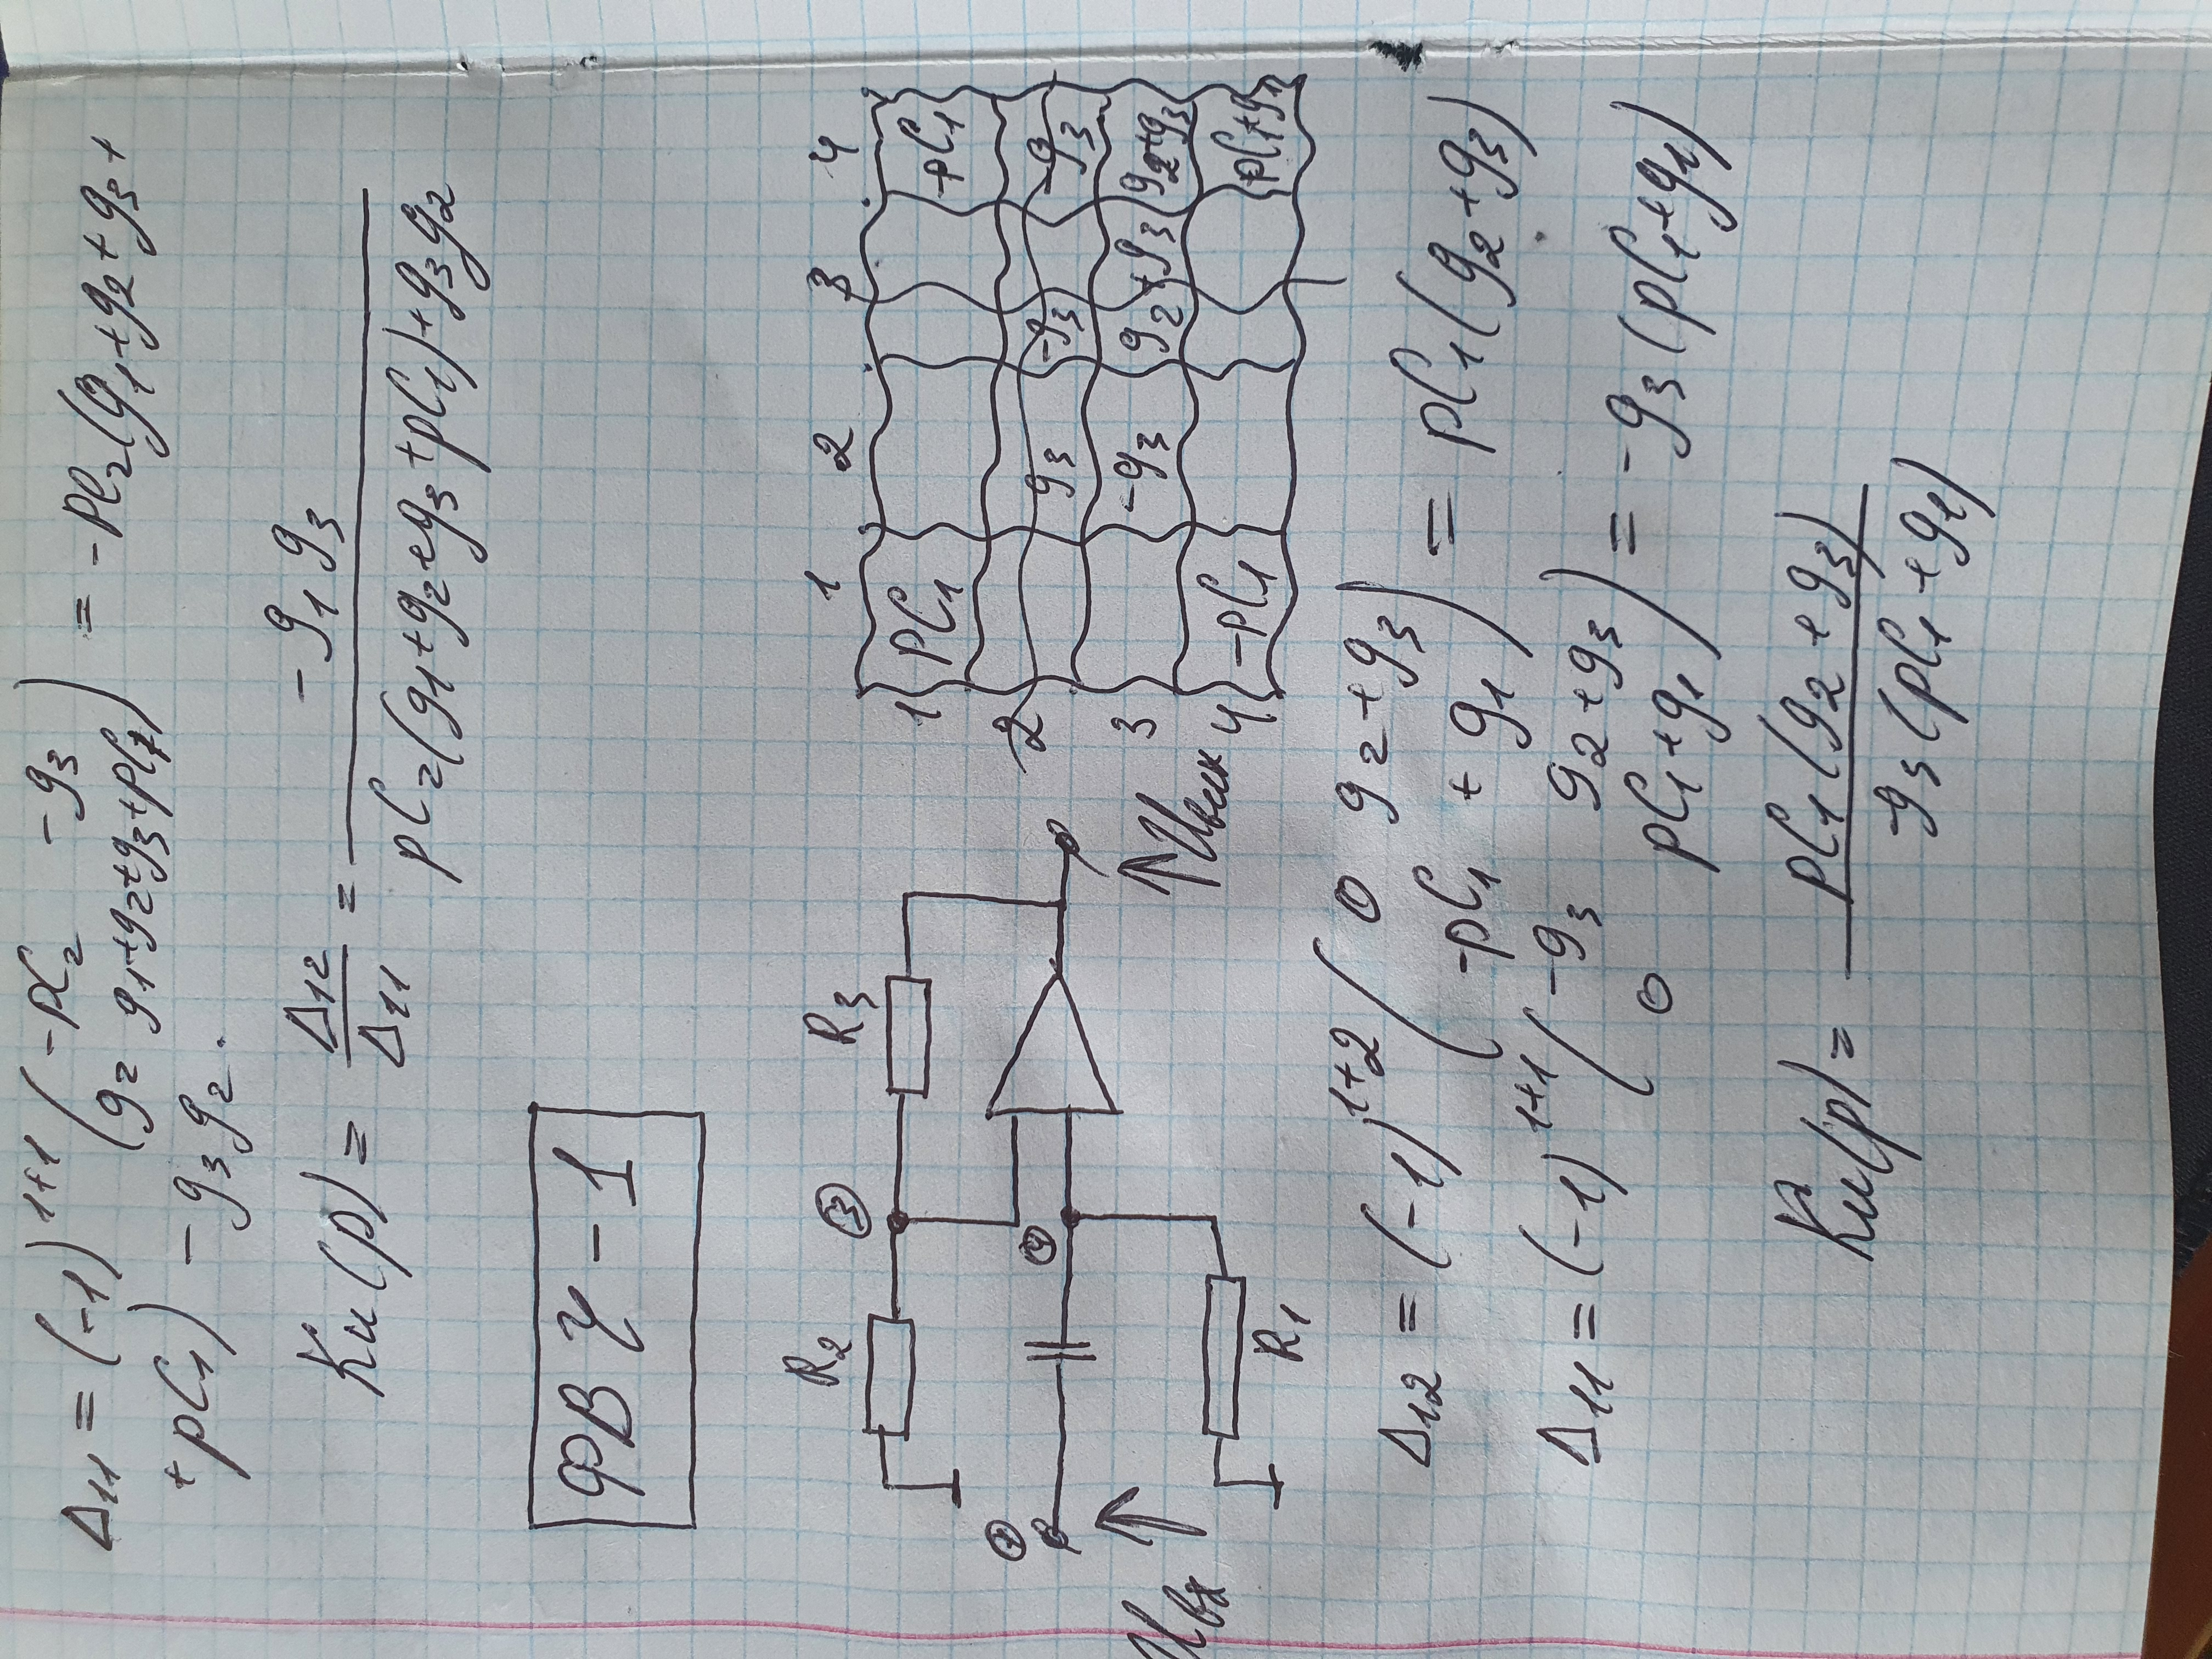
\includegraphics[angle = -90, width=0.8\linewidth]{2.jpg}}
\end{figure}

\begin{figure}[h]
	\center{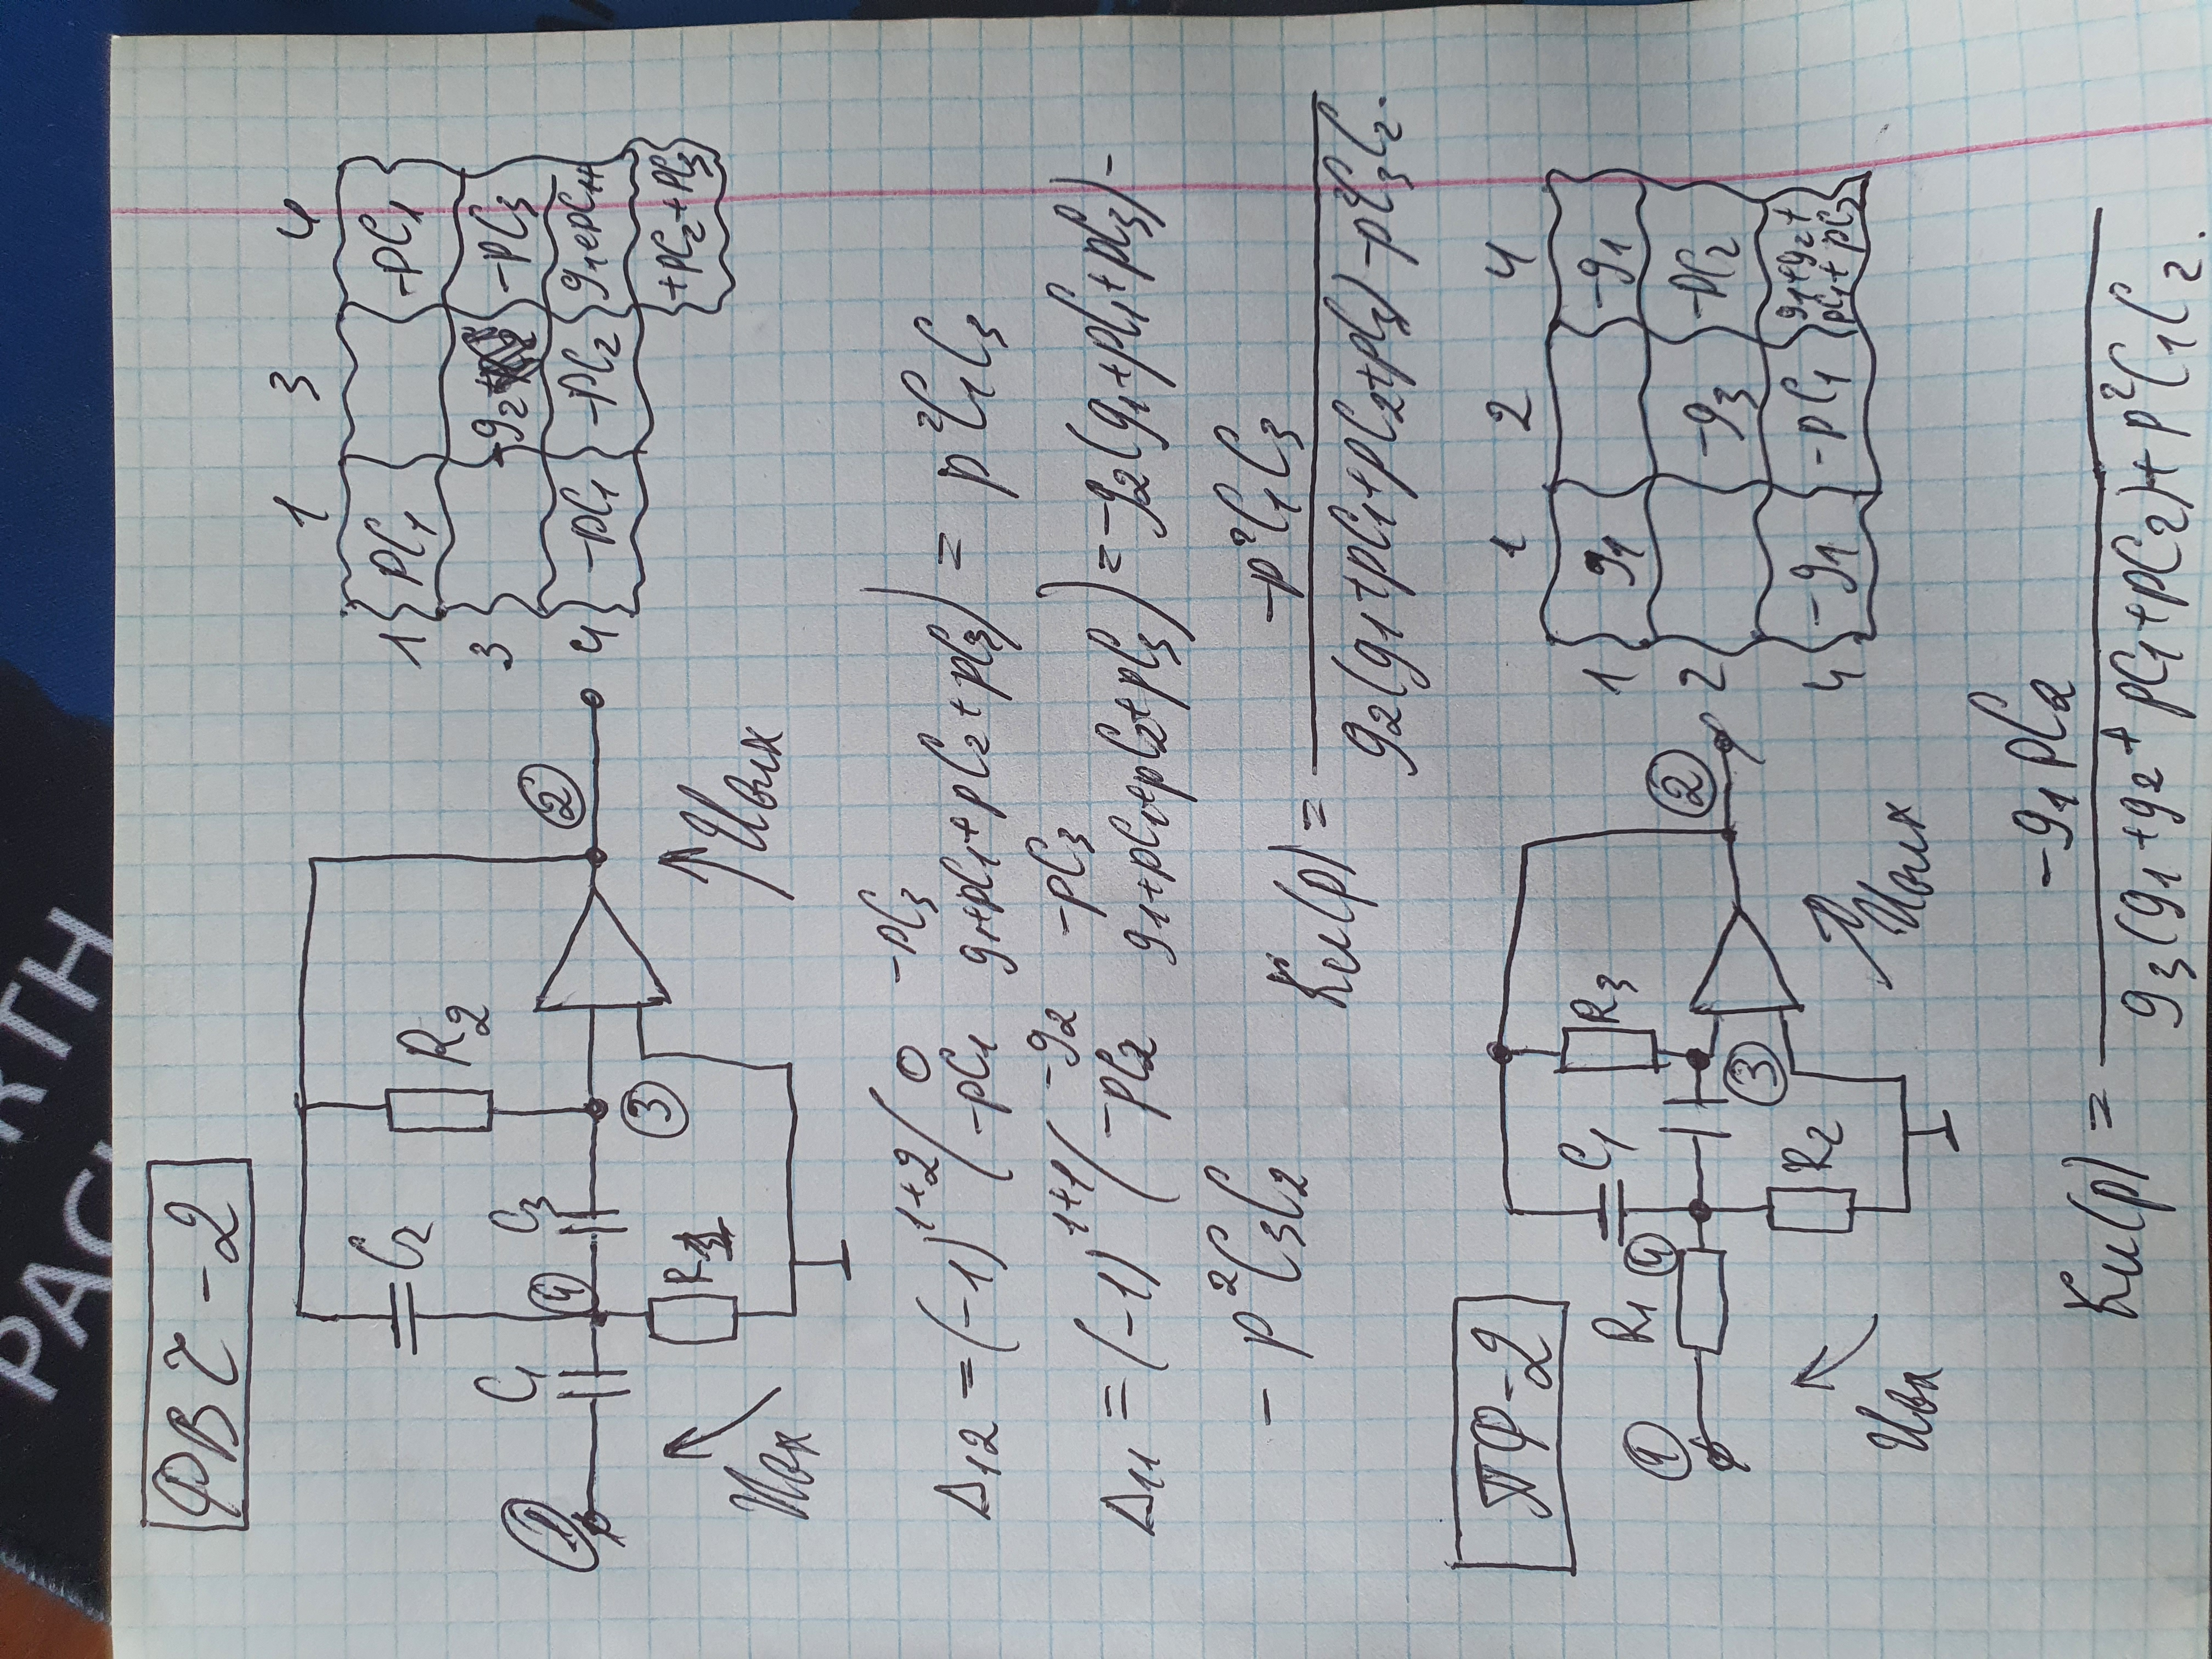
\includegraphics[angle = -90, width=0.8\linewidth]{3e.jpg}}
\end{figure}


\begin{figure}[h]
	\center{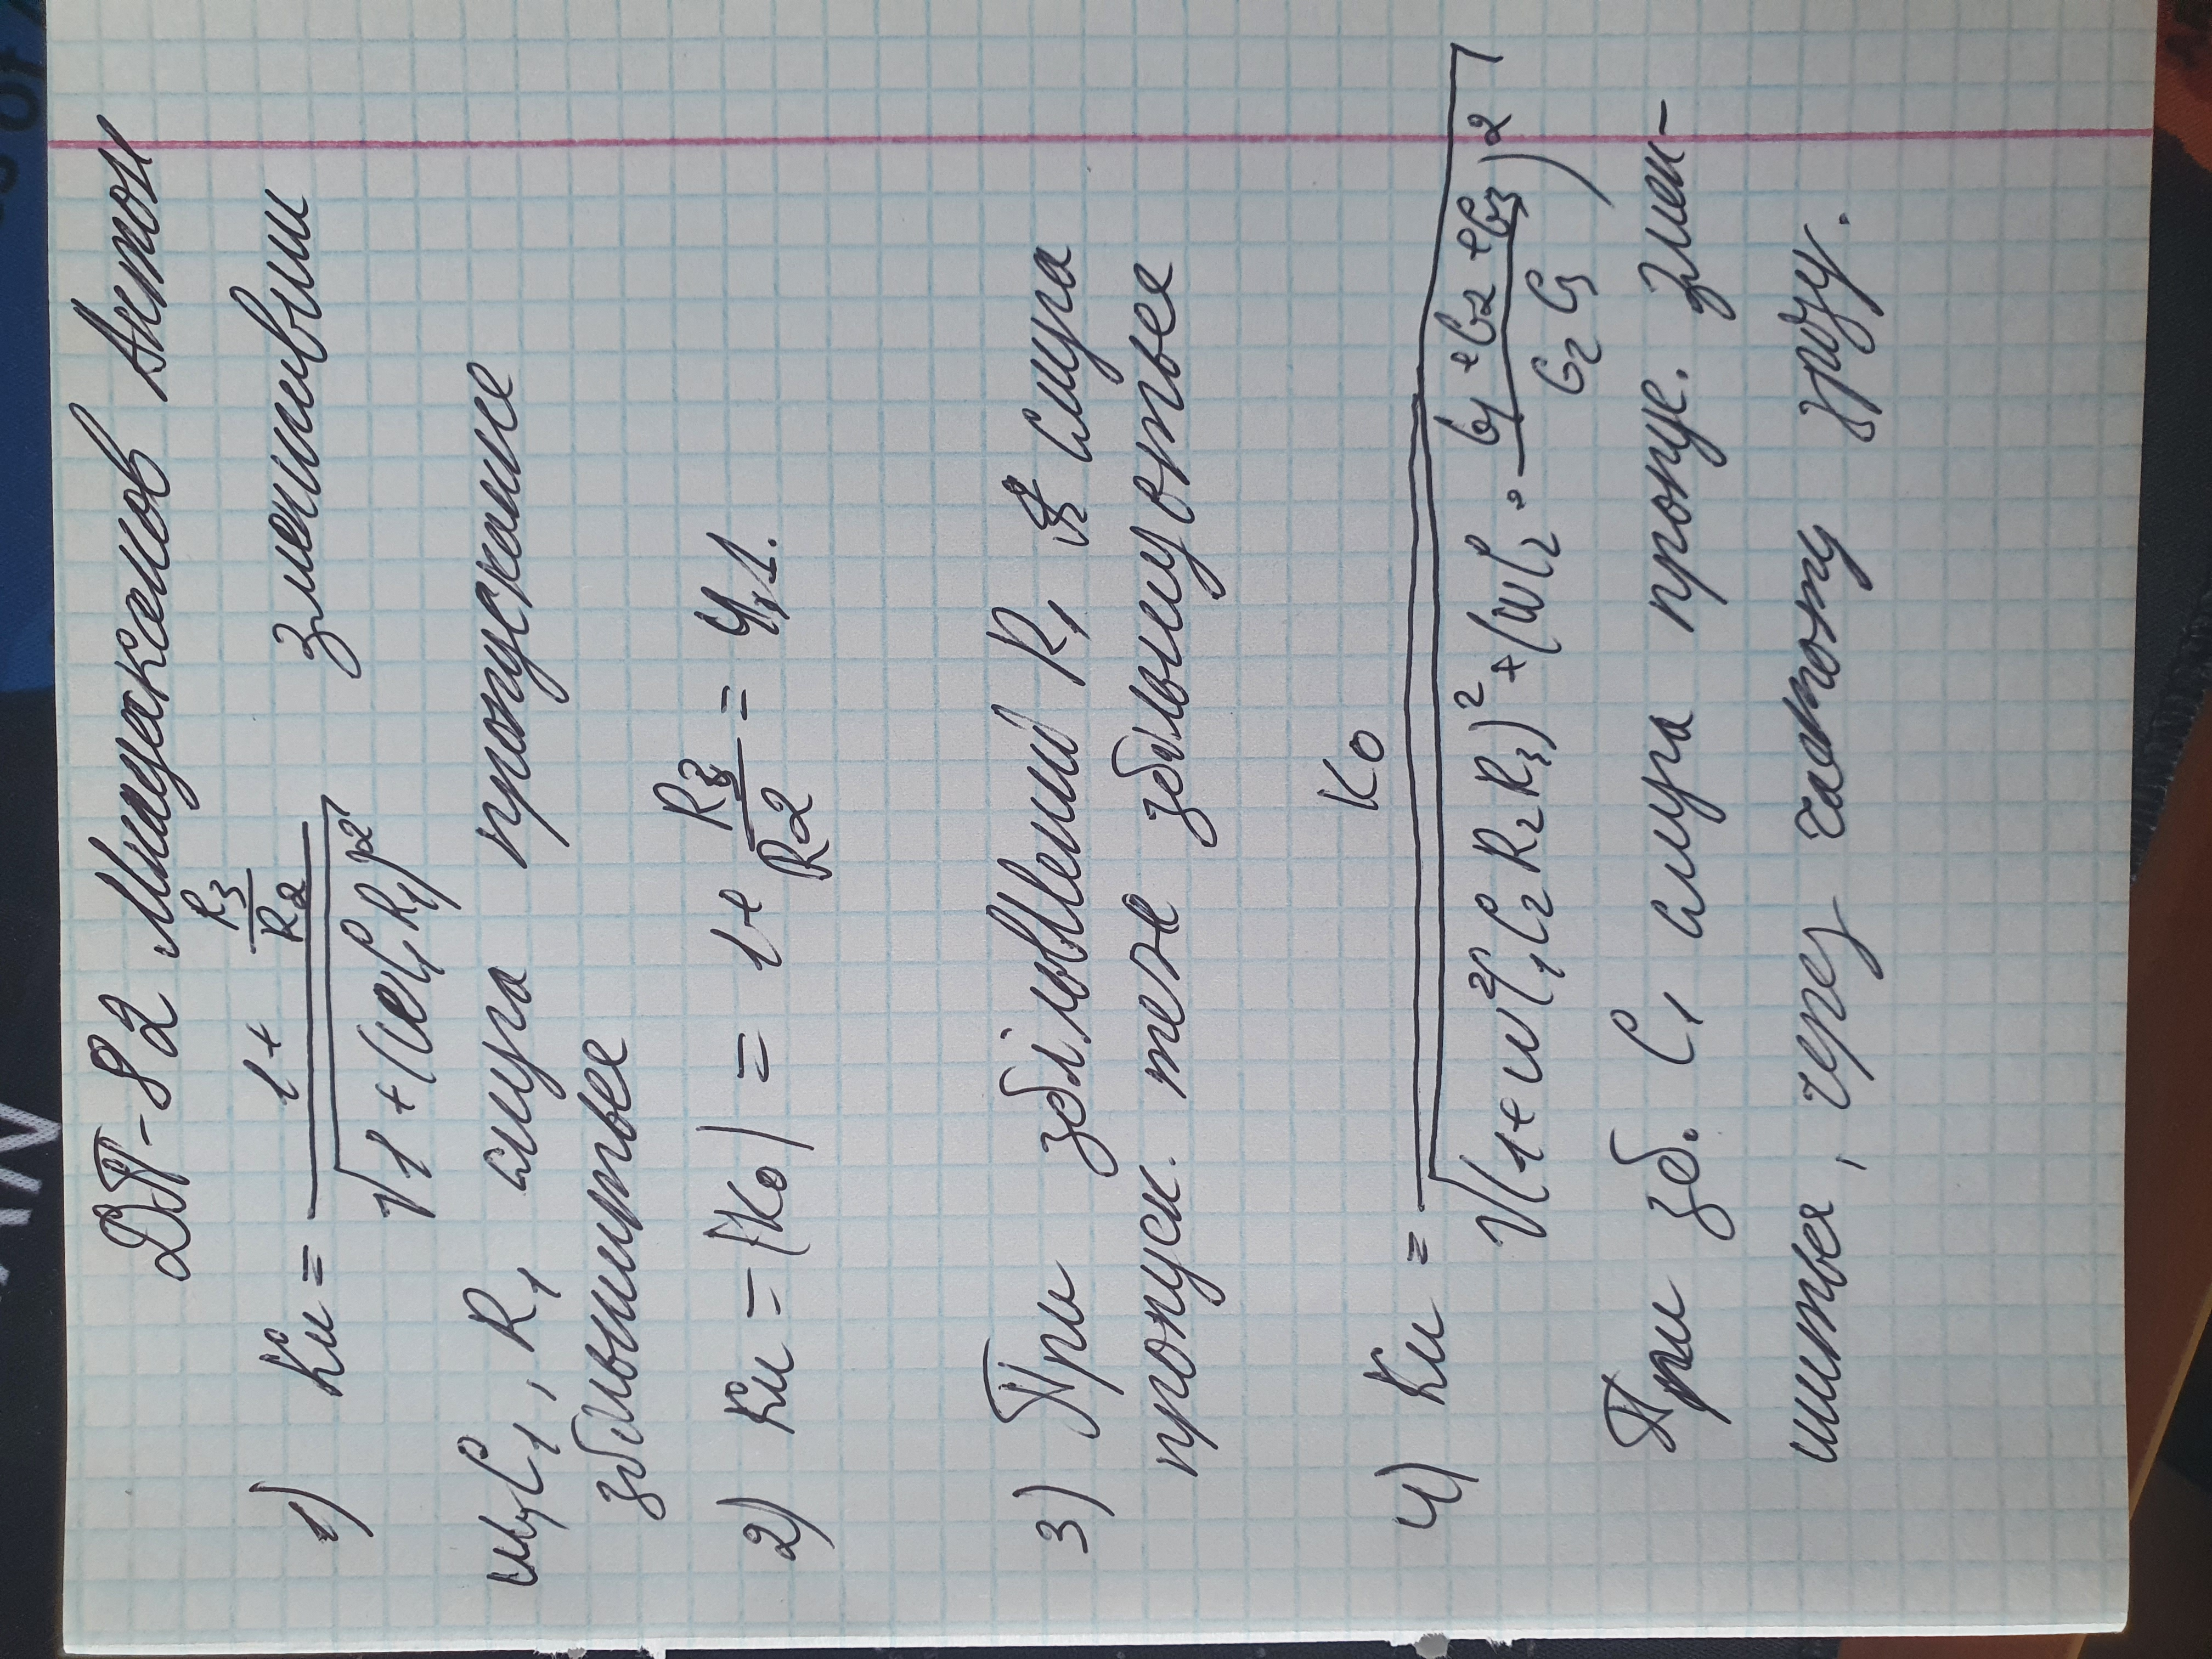
\includegraphics[angle = -90, width=0.8\linewidth]{9.jpg}}
\end{figure}


\end{document}
